\section{Neutrinos for Astrophysics} \label{sec:neutrinos}

Many sources of astrophysical neutrinos exist~\cite{Vitagliano:2019yzm,Gann:2021ndb}, and those in the relevant energy range for xenon experiments are shown in \autoref{fig:nufluxes}. Overall, the flux is dominated by pp solar neutrinos, which will be the leading source of low-energy electronic recoils. Atmospheric neutrinos have the highest energy and can induce sizable nuclear recoils of tens of keV through coherent elastic neutrino-nucleus scattering; their measurement is a goal of the next-generation liquid xenon experiment. A prominent source is $^8$B solar neutrinos as they lie in a sweet spot: their energy is high enough that nuclear recoils are visible in dedicated xenon TPCs, while their flux is so large that a first measurement can be achieved already with LZ and XENONnT.

\begin{figure}[!htbp]
\begin{center}
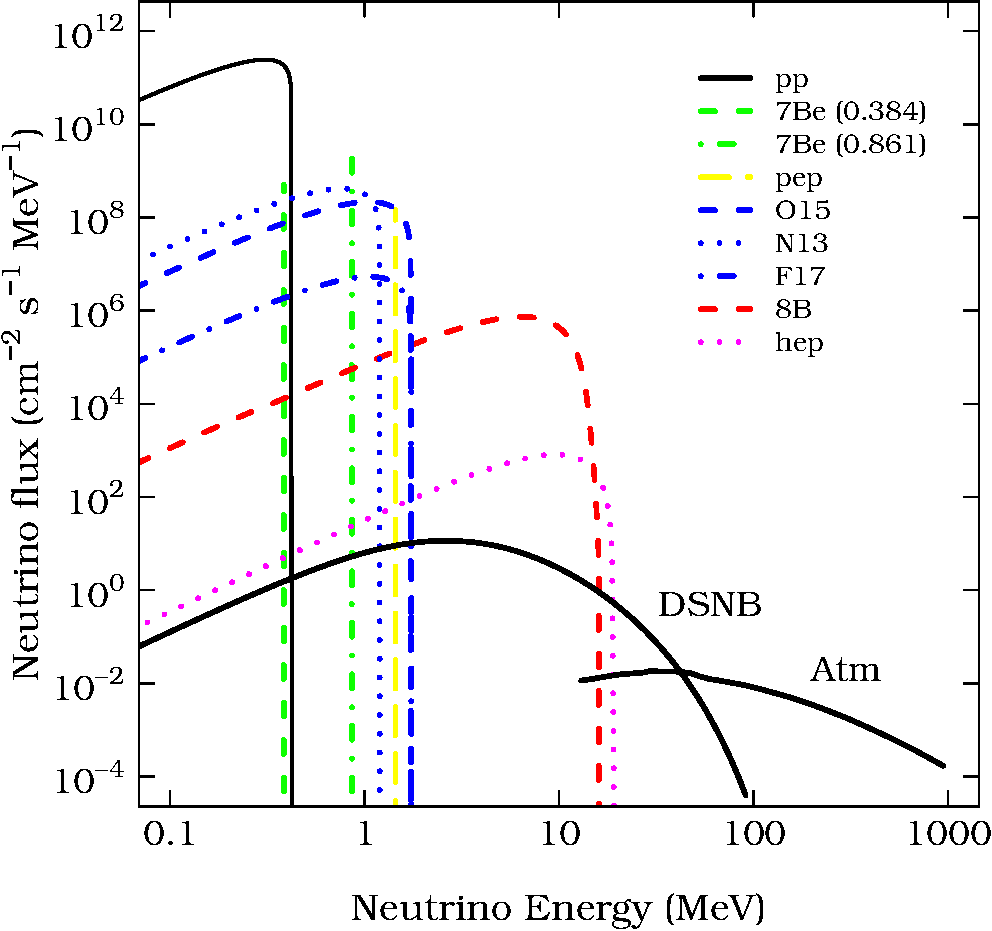
\includegraphics[width=0.99\columnwidth]{fig_nufluxes.pdf}
\caption{Astrophysical neutrino fluxes span many orders of magnitude in flux and energy. This explains the different exposures and energy thresholds required to measure them.}\label{fig:nufluxes}
\end{center}
\end{figure}

A next-generation detector will make important advances in neutrino astrophysics, covering low-energy realms that are out of the reach of experiments such as Hyper-K~\cite{Abe:2018uyc} or DUNE~\cite{Acciarri:2016crz}. This section outlines the scientific scope of the next-generation detector, including solar, atmospheric, and supernova neutrinos, and discusses the unique interaction channels that this detector will be sensitive to. 

\subsection{Neutrino Interactions}

Neutrinos can interact with liquid xenon through Charged Current (CC) and/or Neutral Current (NC) interactions to produce detectable electronic and nuclear recoils. The neutrino-induced rate is
\begin{equation}
\frac{{\rm d}R}{{\rm d}T_R} = \mathcal{N} \times \int_{E_{\nu}^{min}}{\phi\left(E_{\nu}\right) \times \frac{{\rm d}\sigma(E_\nu, T_R)}{{\rm d}T_R} {\rm d}E_\nu}
\end{equation}
where $\mathcal{N}$ is the number of target nuclei or electrons per unit of mass of detector material (for nuclear and electronic recoils, respectively), $\phi\left(E_{\nu}\right)$ is the neutrino flux as a function of the neutrino energy as shown in \autoref{fig:nufluxes}, and $E_{\nu}^{min}$ is the minimum neutrino energy required to generate a recoil at an energy $T_R$. For a nuclear recoil, in the limit where $m_N \gg E_\nu$, the minimum energy is given by 
\begin{equation}
E_{\nu}^{min} = \sqrt{\frac{m_N T_R}{2}},
\end{equation}
whereas in the case of an electronic recoil, it is given by 
\begin{equation}
E_{\nu}^{min} = \frac{1}{2}\left( T_R + \sqrt{T_R\left( T_R + 2m_e \right)}\; \right)
\end{equation}

The differential cross section depends on the nature of the interaction. In the next two sections, we discuss Coherent Elastic Neutrino-Nucleus Scattering and the Electroweak interaction, which constitute the major contributions to the potential detectable signal for liquid xenon detectors.

\subsubsection{Coherent Elastic Neutrino-Nucleus Scattering} \label{sec:cevns}

In the Standard Model, elastic neutrino-nucleon scattering proceeds only through neutral current interaction with the exchange of a $Z$-boson. The resulting differential neutrino-nucleus cross section as a function of the nuclear recoil energy $T_R$ and the incoming neutrino energy $E_\nu$ is
\begin{equation}
\begin{split}
\frac{{\rm d}\sigma(E_\nu, T_R)}{{\rm d}T_R} = \frac{G^2_f}{\pi} m_N  \left( Z g_v^p + N g_v^n \right)^2 \\
\times \left(1 - \frac{m_NT_R}{2E^2_{\nu}}
\right) F^2(T_R)
\end{split}
\end{equation}
where $m_N$ is the target nucleus mass, $G_f$ is the Fermi coupling constant, $N$ the number of neutrons, $Z$ the number of protons, $g_v^n = -1/2$, and $g_v^p = 1/2 - 2 \sin^2 \theta_w$, where $\theta_w$ the Weak mixing angle. Because $\sin^2{\theta_w}\simeq 0.23$, the cross section scales roughly with the number of neutrons squared. The nuclear form factor $F(T_R)$ describes the loss of coherence due to the internal structure of the nucleus. For momentum transfers less than the inverse of the size of the nucleus, the coherence condition is largely satisfied and $F(T_R) \rightarrow 1$. In lieu of experimental data on the neutron distribution in the nucleus, a typical parameterization is the Helm form factor~\cite{Helm:1956zz} that is also commonly used for WIMP direct detection~\cite{Engel:1991wq, Lewin:1995rx}.

\begin{figure}[!htbp]
\begin{center}
   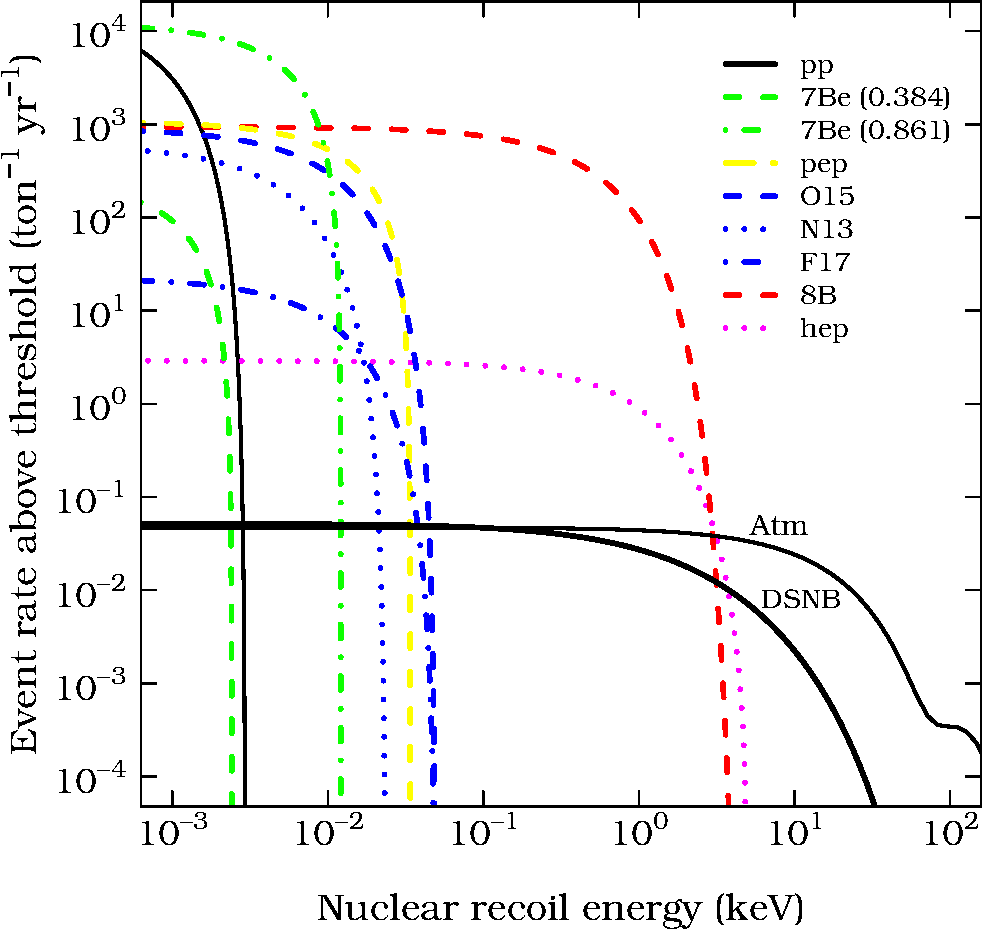
\includegraphics[width=0.99\columnwidth]{fig_nurates.pdf}
   \caption{Nuclear recoil event rates from astrophysical neutrinos via CEvNS. $^8$B solar neutrinos are expected to be measured first in the upcoming LZ and XENONnT experiments. The detector proposed here targets a precision measurement of that flux, and a first measurement of the atmospheric neutrino flux.}\label{fig:nurates}
\end{center}
\end{figure}

In effect, this Coherent Elastic Neutrino-Nucleus Scattering (CEvNS)~\cite{Akimov:2017ade} increases the cross section for heavy nuclei such as xenon, while pushing the recoil energy spectrum to small energies of keV or less. Given the excellent performance of liquid xenon detectors at such low energies, this channel thus opens the possibility to detect neutrinos from astrophysical sources with a target mass that is modest in comparison to other neutrino detectors, see \autoref{fig:nurates}. In addition to providing the possibility to measure some astrophysical neutrino sources for the first time, the fact that this interaction is flavor-independent provides complementary information for sources that have been measured by other neutrino detectors~\cite{Cabrera:1984rr,Krauss:1985pf}.

\subsubsection{Electroweak interaction}\label{sec:ewinteraction}

The neutrino-electron electroweak interaction proceeds through both Charged Current ($W$-boson exchange) and Neutral Current ($Z$-boson exchange) interactions. In the free electron approximation, the resulting differential neutrino-electron cross section as a function of the electronic recoil energy $T_R$ and the incoming neutrino energy $E_\nu$ is
\begin{align*}
\frac{{\rm d}\sigma(E_\nu, T_R)}{{\rm d}T_R} & = \frac{G^2_f m_e}{2 \pi} \Bigg[ \Bigg. \left( g_v + g_a \right)^2 \\
 & + \left( g_v - g_a \right)^2 \left(1 - \frac{T_R}{E_{\nu}}\right)^2 + \left(g_{a}^{2} - g_{\nu}^{2} \right) \frac{m_e T_R}{E_{\nu}^2}\Bigg. \Bigg]
\end{align*}
where $m_e$ is the electron mass, $G_f$ is the Fermi coupling constant, $g_v = 2\sin^2{\theta_w} - 1/2$ and $g_a = 1/2$ are respectively the vectorial and axial coupling, and $\theta_w$ is the weak mixing angle. In the context of $\nu_e + e \rightarrow \nu_e + e$ scattering, the interference coming from the addition of the charge current leads to a shift in axial and vectorial couplings such as: $g_v \rightarrow g_v +1$ and  $g_a \rightarrow g_a +1$. This is then contributing to enhance the $\nu_e + e \rightarrow \nu_e + e$ scattering cross section with respect to the $\nu_{\tau, \mu} + e \rightarrow \nu_{\tau, \mu} + e$ cross section by about one order of magnitude. Further, neutrino oscillations also are an important factor that needs to be taken into account to properly calculate neutrino-induced event rates.

Low-energy electronic recoil starts to deviate from the simple free electron approximation. Below few keV, it is important to include the stepping of atomic shells and atomic binding. This has been included into the calculation by using the Relativistic Random Phase Approximation (RRPA) as presented in~\cite{Chen:2016eab}. The inclusion of these atomic effects result in a reduction of the neutrino-induced electronic recoil event rate below $\sim 5$~keV. Importantly, this reduces the neutrino background in the $[2–10]\1{keV}$ energy range by $\sim$22\%. \autoref{fig:electronrates} shows the electronic recoil event rate for different neutrino flux contributions including the RRPA corrections. The wavy features in the energy spectra are directly related to the RRPA corrections.

\subsection{Solar Neutrinos}\label{sec:solarneutrinos}

Experimental studies of solar neutrinos date back to over half of a century ago~\cite{Bahcall:1976zz}. The primary goal of these experiments is to measure the different components of the solar neutrino flux, in order to provide an understanding of the physics of the solar interior. Many different types of solar neutrino experiments were operated, and they have evolved in their size and scientific scope since the original experiments~\cite{Robertson:2012ib}. The combination of all solar neutrino data with terrestrial experiments that study neutrinos in the same energy range has led to the LMA-MSW solution to neutrino flavor transformation from the Sun to the Earth~\cite{deHolanda:2002dko}. With this solution, at low energies $\lesssim 5\1{MeV}$, vacuum oscillations describe the neutrino flavor transformation, and the electron neutrino survival probability is $\gtrsim 50\%$. At energies $\gtrsim 5\1{MeV}$, matter-induced transformations describe the flavor transformation, with a corresponding survival probability of $\gtrsim 1/3$. 

However, in spite of all the theoretical and experimental progress in the field of solar neutrino physics over the past several decades, there are still outstanding questions that surround some of the data. For example, three experiments (Super-Kamiokande, SNO, and Borexino) that are sensitive to electronic recoils from neutrino-electron elastic scattering find that, at electronic recoil energies of a few MeV, the data are $\sim 2\sigma$ discrepant relative to the prediction of the best-fitting LMA-MSA solution. In addition, the recent measurement of the solar mass-squared difference from solar neutrino data, in particular from the day-night Super-Kamiokande data~\cite{Abe:2016nxk}, is discrepant at the $\sim 2 \sigma$ level relative to that measured by KamLAND~\cite{Gando:2010aa}. Non-standard interactions provide a possible solution to this discrepancy~\cite{Liao:2017awz}. 

\begin{figure}[!htbp]
\begin{center}
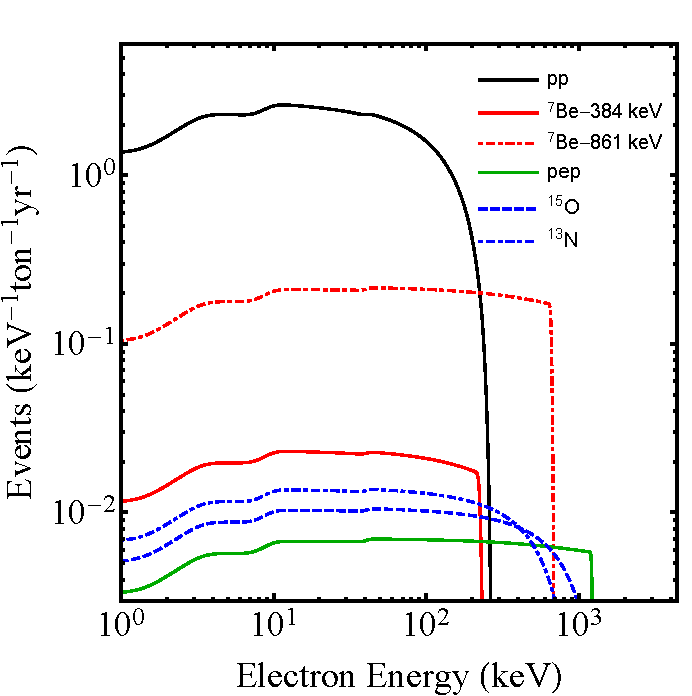
\includegraphics[width=0.99\columnwidth]{fig_spectrum_smear.pdf}
\caption{Electronic recoil scattering rates from solar neutrinos. The step-wise decrease in event rate towards low energies corresponds to the energy levels of electrons in the xenon atom.}\label{fig:electronrates}
\end{center}\end{figure}

Another outstanding question relates to the measured neutrino flux, and how it is able to inform the physics of the solar interior. There is a long-standing problem with standard solar models (SSMs) and predictions of the abundances of heavy elements, or metals, in the Sun. Older abundance calculations~\cite{Grevesse:1998bj} relied on many simplifying assumptions, but nevertheless fit solar observables well, in particular helioseismology data. More recent calculations however~\cite{Asplund:2009fu}, while more sophisticated in construction, were ultimately worse fits to the data~\cite{Asplund:2009fu,Scott:2014lka,Scott:2014mka,Grevesse:2014nka}. These calculations are referred to as high-Z and low-Z models respectively, according to their relative predicted metallicities. Their disagreement is known as the solar abundance problem~\cite{Serenelli:2009yc}, and has not yet been resolved. A global analysis of all solar neutrino fluxes remains inconclusive~\cite{Bergstrom:2016cbh}. A step towards resolving this problem will be to accurately measure the flux of solar neutrinos from the CNO nuclear fusion cycle, first achieved by Borexino~\cite{Agostini:2020mfq}, which is possible with the experiment discussed here (\autoref{sec:cno}).

\subsubsection{Boron-8 Solar Neutrinos (NR)}

Combined with the neutrino-electron scattering data from SNO, Super-Kamiokande and Borexino, precision measurements of $^8$B neutrino induced CEvNS in a next-generation liquid xenon detector will constrain the $\nu_e$ survival probability in the 5--15 MeV range. A significant deficit from the theoretical prediction can be interpreted as evidence of active-to-sterile neutrino oscillation~\cite{Billard:2014yka}. A next-generation liquid xenon detector will provide an independent measurement of the neutral current component of the solar $^8$B neutrino flux, with an expected event rate of $\sim 90$ events per tonne-year~\cite{Aalbers:2016jon}, measured to be right in between that predicted by the low and high metallicity Standard Solar Model~\cite{Agostini:2017cav,Agostini:2018uly,Aprile:2020thb}.

\subsubsection{Hep Solar Neutrinos (NR)}

A future next-generation detector may detect neutrinos from the minor branch of the pp chain that generates the most energetic neutrinos via the reaction $^{3}$He + p $\rightarrow ^{4}$He + e$^-$ + $\nu_e$. Along with $^{8}$B neutrinos, neutrinos from this hep reaction also undergo adiabatic conversion in the solar interior. Neutrinos from the hep reaction have not been directly identified in solar neutrino experiments the best upper bound from the SNO experiment is $\sim 4$ times greater than the SSM prediction~\cite{Aharmim:2006wq}. 

\subsubsection{pp Solar Neutrinos (ER)}\label{sec:ppneutrinos}

The possibility to use liquid xenon as a low-energy solar neutrino detector by means of $\nu + e$ scattering was suggested in~\cite{Suzuki:2000ch} but only now is about to being realized. A next-generation liquid xenon detector will provide a new, high-precision observation of the electronic recoil energy spectrum induced by elastic scattering of pp neutrinos, see \autoref{fig:electronrates}. This, in turn, will improve measurements of the Sun's (neutrino) luminosity. The pp neutrino flux was first indirectly identified as a component of the Gallium data, and Borexino was the first experiment to make a measurement of the spectral energy distribution of electronic recoil events induced by pp neutrinos~\cite{Smirnov:2015lxy}. The Borexino measurement uncertainty on this component is now down to $\lesssim 10\%$~\cite{Agostini:2018uly}. Further improving upon the measurement of this component will better constrain the ``neutrino luminosity'' of the Sun because pp neutrinos account for 86\% of all solar neutrino emission~\cite{Bahcall:2001pf}. Projections for a next-generation xenon experiment indicate that the pp neutrino flux can be measured to 0.15\% uncertainty with 300 tonne-years of exposure. Combined with a 1\% measurement of the next-largest component, $^7$Be, such a detector could ultimately achieve 0.2\% uncertainty in the neutrino-inferred solar luminosity~\cite{Aalbers:2020gsn}. This will also have the important consequence of constraining alternative sources of energy production in the solar interior~\cite{Newstead:2018muu}. 

\subsubsection{CNO Neutrinos (ER)}\label{sec:cno}

The flux of CNO neutrinos from the Sun makes up less than 1\% of the Sun's total neutrino luminosity but is sensitively dependent on the solar metallicity, with higher metallicity models predicting a higher CNO component. A precise measurement of the CNO flux would provide the necessary information to discriminate between the low and high-Z calculations, thereby resolving the solar abundance problem directly. The very first measurement of CNO neutrinos was achieved recently by Borexino~\cite{Agostini:2020mfq}, though with insufficient statistics to yet conclusively resolve the abundance problem. 

Due to the small CNO luminosity fraction, measuring the CNO flux in a xenon TPC will require large experimental exposures and well controlled backgrounds. A next-generation liquid xenon detector would be capable of measuring the $^{13}$N and $^{15}$O fluxes individually (20-25\%) even in the presence of the $\nu\nu\beta\beta$ decay background from $^{136}$Xe~\cite{Aalbers:2020gsn}. Significant improvements to the precision of these measurements can be achieved through depletion of the natural xenon target from the $^{136}$Xe isotope~\cite{Newstead:2018muu}, while negating the possibility of a $0\nu\beta\beta$ search (\autoref{sec:0nubb}). Hence, both a natural xenon target and a $^{136}$Xe-depleted target provide exciting physics opportunities for a next-generation liquid xenon detector.

\subsubsection{Neutrino Capture on Xenon-131 and Xenon-136}

Solar neutrinos may also be observed through the neutrino capture process on xenon: $\nu_e + \,^{A}_{54}\textrm{Xe} \to \,^{A}_{55}\textrm{Cs}^{(*)} + e^{-}$~\cite{Georgadze:1997zv}. The isotopes $^{131}$Xe and $^{136}$Xe have sufficiently low reaction thresholds of $Q=355$~keV and $Q=90.3$~keV for capture of all solar neutrino species. The prompt electron gives an electronic recoil with an energy that is offset from that of the captured neutrino as $E_e = E_\nu-Q-E_{\rm ex}$, where $E_{\rm ex}$ is the excitation energy of the resulting Cs nucleus.

The possibility of tagging neutrino capture events which populate excited states in the product Cs  nuclei has been explored in~\cite{Haselschwardt:2020ffr}. The emission of $\gamma$-rays and/or conversion electrons during relaxation of the excited nuclear state in conjunction with the primary fast electron provides opportunities for background rejection. 

An especially high suppression of background can be achieved if a delayed coincidence signature in the Cs de-excitation could be exploited. The product isotopes $^{131}$Cs and $^{136}$Cs are unstable with half-lives 9.7~d and 13.0~d, respectively. Detection of the corresponding electron-capture and $\beta$-decay signatures which occur long after the initial capture event may also be possible. With abundances of 21.2\% and 8.9\%, one expects 0.6 and 0.7 neutrino capture events per tonne of natural Xe per year on $^{131}$Xe and $^{136}$Xe, respectively~\cite{Haselschwardt:2020ffr}.

\subsection{Atmospheric Neutrinos (NR)}\label{sec:atmnu}

The collisions of cosmic rays in the atmosphere produce neutrinos over a wide range of energies. A precise determination of this atmospheric neutrino flux depends on several factors, including the cosmic-ray flux at the top of the Earth's atmosphere, the propagation of cosmic rays through the atmosphere, and the decay of the mesons and muons as they propagate though the atmosphere to Earth's surface. Since the flavors of neutrinos that are produced in the decays are known, theoretical models accurately predict the ratio of the flavor components of neutrinos across all energies. However, the normalizations of the fluxes differ depending upon the theoretical input. 

\begin{figure}[!htbp]
    \centering
    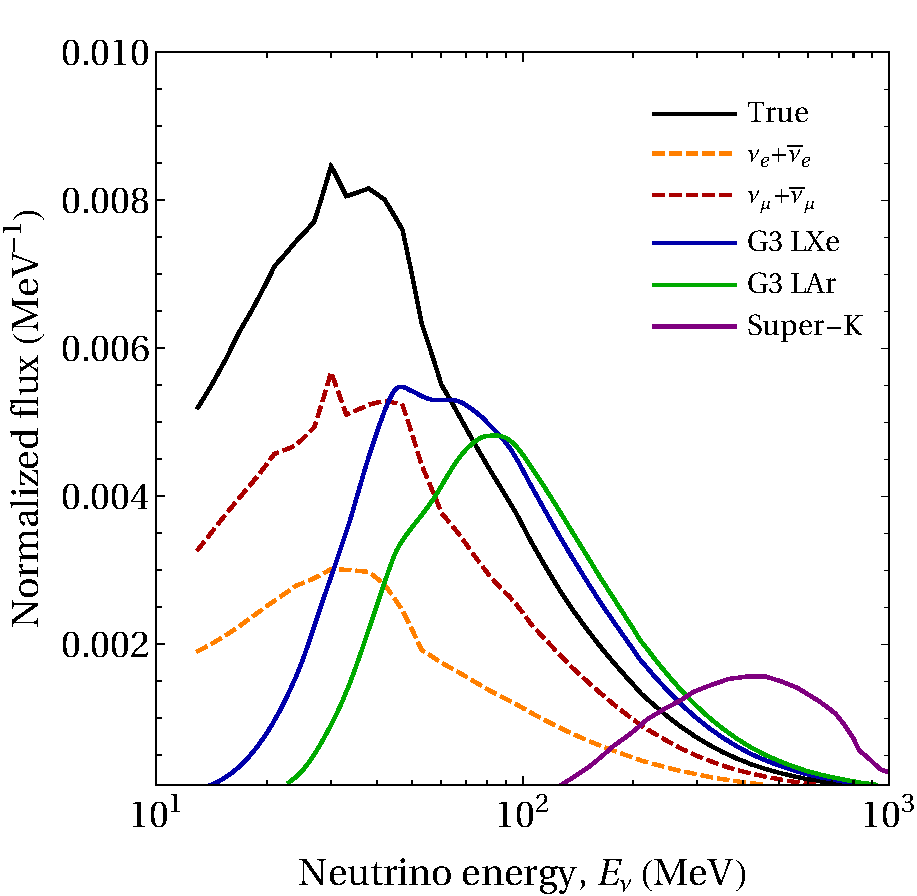
\includegraphics[width=\columnwidth]{fig_fluxcomp.pdf}
    \caption{The differential fluxes of atmospheric neutrinos that are accessible by various experiments, normalized such that the area under the curves is equal to unity. The flux accessible to a next-generation xenon experiment (labeled G3 LXe) is shown in blue, and reaches much lower in energy than Super-Kamiokande currently does (shown as solid violet). Figure from~\cite{Newstead:2020fie}.}
    \label{fig:atmneutrino}
\end{figure}

While the atmospheric neutrino flux for energies $\gtrsim1\1{GeV}$ has been well studied by the aforementioned experiments, the low-energy flux of atmospheric neutrinos, $\lesssim100\1{MeV}$, is difficult to both model and measure~\cite{Battistoni:2005pd}. The resulting energy spectrum of neutrinos corresponds to that from muon and pion decay at rest, but the absolute normalization of the flux is less well constrained, due to uncertainties that arise from several uncertain physical processes. A next-generation dark matter detector will measure this neutrino flux at so-far unexplored low energy, see \autoref{fig:atmneutrino}. Measuring atmospheric neutrinos will require an exposure of order 700~tonne-years~\cite{Newstead:2020fie}, thus providing a benchmark target exposure for a next-generation liquid xenon observatory.

\subsection{Supernova Neutrinos (NR)}\label{sec:supernovaneutrinos}

The next supernova event in the Milky Way or in nearby galaxies will provide unprecedented information on the physics of neutrino propagation from the supernova core~\cite{Janka:2006fh,Janka:2012wk}. For example, large water Cherenkov detectors such as Super-Kamiokande will measure thousands of events, mostly through the charged-current inverse beta decay channel, and hundreds of events through various other elastic and inelastic channels~\cite{Scholberg:2012id}. Dark matter detectors can play an important role in supernova neutrino astrophysics through their sensitivity to supernova neutrinos via coherent elastic scattering, yielding complementary information for example on the nature of stellar collapse and the explosion energy of the supernova~\cite{Freedman:1977xn}.

\subsubsection{Galactic Supernova Neutrinos}

Current and future liquid xenon dark matter detectors are uniquely sensitive to neutrinos of all flavors through CEvNS~\cite{Horowitz:2003cz,XMASS:2016cmy}, whether from core-collapse (Type~II)~\cite{Chakraborty:2013zua,Lang:2016zhv} or thermonuclear runaway fusion (Type~Ia)~\cite{Raj:2019sci}. This provides a calorimetric measurement of the explosion energy going into neutrinos, independent of oscillation effects~\cite{Lang:2016zhv}. The physics available with the statistics collected by a next-generation liquid xenon detector would complement that of larger, dedicated neutrino observatories. In a next-generation detector, there are $\mathcal{O}(100)$ expected events from a core-collapse supernova within 10~kpc of Earth~\cite{Lang:2016zhv}.

CEvNS is the primary detection interaction from galactic neutrinos in liquid xenon detectors, but charge current reactions are also possible. A supernova within 10~kpc could produce a handful of charge current interactions in a next-generation detector, particularly interacting with the $^{136}$Xe isotope~\cite{Pirinen:2018gsd,Ydrefors2015}. Even the large water Cherenkov veto volumes that typically surround these detectors may record notable supernova neutrino event rates~\cite{Litvinovich:2017smi}. 

Also possible are inelastic neutral and charge current interactions of the supernova neutrinos with the xenon nuclei in which, depending on the incident neutrino energy, the final state nucleus is left in an excited state, with an excitation energy beyond its single or multiple neutron emission thresholds~\cite{Bhattacharjee:2020rhs,Bhattacharjee:2020qrj}. The neutrons resulting from de-excitation of the final state nuclei would undergo multiple scattering on the xenon nuclei themselves. This in turn yields further xenon recoils in addition to those caused by the direct CEvNS process. Indeed, the total xenon recoil spectrum can be dominated~\cite{Bhattacharjee:2020qrj} by the contribution from these neutrino-induced neutrons ($\nu$I$n$) at relatively high recoil energies beyond $\sim20\1{keV}$ where the CEvNS recoil spectrum rapidly falls off with increasing recoil energy. 

Observations of astrophysical neutrinos are complementary to terrestrial experiments which are sensitive to MeV-scale neutrinos. The recent detection of CEvNS has provided novel bounds on new physics, for example in the form of kinetic mixing, hidden sector models, flavor models, and sterile neutrinos~\cite{Akimov:2017ade}. Future measurements of supernova neutrinos at dark matter detection experiments can improve on this sensitivity, providing further information on new physics models (see also \autoref{sec:otherstuff}).

\subsubsection{Pre-Supernova Neutrinos}

\begin{figure}[!htbp]
    \centering
    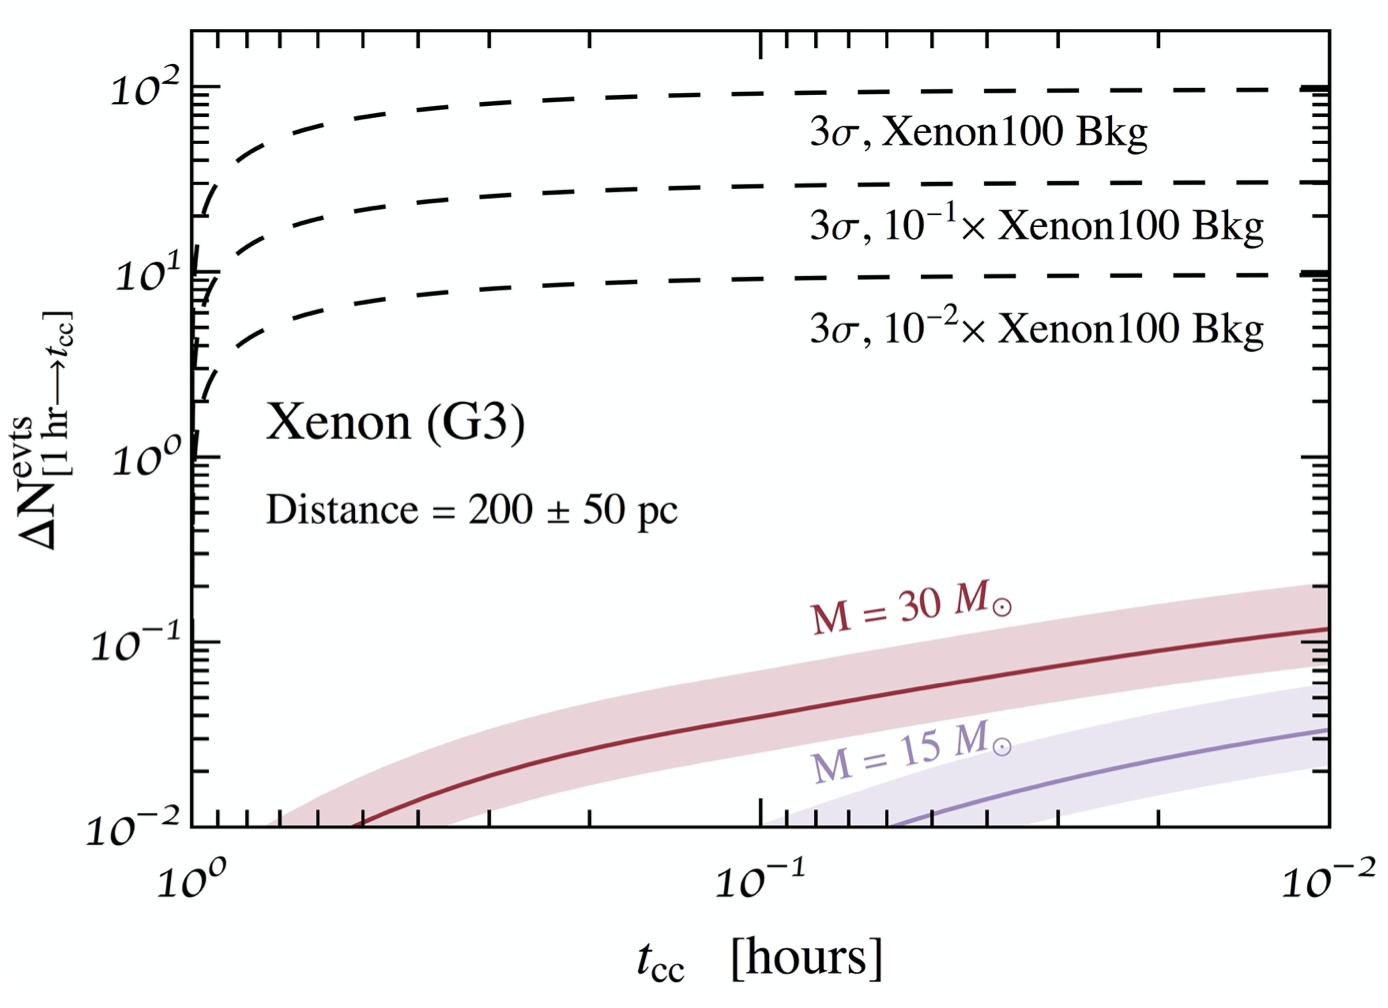
\includegraphics[width=\columnwidth]{fig_presupernova_neutrinos.png}
    \caption{For a next-generation liquid xenon dark matter experiment with an assumed target mass of 50~tonnes, the expected number of pre-supernova neutrinos above the detection threshold is shown for two different stellar masses at a distance of 200~pc. Figure from~\cite{Raj:2019wpy}.}
    \label{fig:pre_sn}
\end{figure}

In the event of a near-Earth ($d <$~kpc) core-collapse supernova, future liquid xenon detectors will also be sensitive to neutrinos of all flavors that are emitted by a massive star in its silicon-burning stage, a few hours \textit{prior to} core collapse~\cite{Odrzywolek:2003vn,Odrzywolek:2004em}. Due to lower stellar temperatures before collapse, these ``pre-supernova" neutrinos are $\mathcal{O}$(10) softer than supernova neutrinos, and therefore require low thresholds for detection~\cite{Kato:2020hlc}. \autoref{fig:pre_sn} indicates that a next-generation liquid xenon experiment operating at 0.1 keV energy threshold would detect, in a 12 hour window prior to collapse, $\mathcal{O}$(100) pre-supernova neutrinos from a massive star 200\,pc away, e.g.~Betelgeuse~\cite{Raj:2019wpy}. Such a detection would constitute the first measurement of the final stages of stellar evolution, and provide a valuable warning before the explosion.

\subsubsection{Supernova Early Warning System} 

In order to be prepared for the next supernova, the Supernova Early Warning System (SNEWS) was developed~\cite{snewsweb}. SNEWS is an inter-experiment network to prepare and provide an early warning for Galactic supernovae: In contrast to the optical signal, neutrinos basically free-stream from the collapsing star and thus reach Earth minutes, hours or even days before the optical counterpart becomes visible. Therefore, by detecting supernova neutrinos, an early alert can be sent to astronomers to facilitate early observations of the Supernova~\cite{Antonioli:2004zb}. SNEWS is in the process of being revamped and amplified to SNEWS2.0 which will have a larger physics reach~\cite{Kharusi:2020ovw,Baxter:2021aaa}. The next-generation detector discussed here will be able to contribute to this network.

\subsubsection{Diffuse Supernova Neutrinos}

In addition to the yield from a Galactic supernova event, an exciting prospect is the detection of the diffuse supernova neutrino background (DSNB)~\cite{Lunardini:2010ab,Beacom:2010kk}, i.e.~the neutrinos emitted from past supernovae occurring across the universe. Modern predictions put this flux at approximately $6\1{cm^{-2}}s^{-1}$~\cite{Horiuchi:2008jz}, including contributions from all neutrino flavors. In addition to being a probe on supernova physics, the diffuse supernova neutrino background is an independent probe of the local core-collapse supernova and cosmic star formation rate~\cite{Hopkins:2006bw}. Although this signal has not yet been directly detected, there are strong upper bounds on the $\bar{\nu}_e$ component of the flux from Super-Kamiokande~\cite{Bays:2011si}. The best predictions for the flux of all flavors, with an expected event rate of $\sim 0.05$ events per tonne-year, implies that liquid xenon dark matter detectors with exposures $\sim 1000$~tonne-year may have discovery potential to this signal above known backgrounds~\cite{Strigari:2009bq}. 

\subsection{Other Neutrino Physics}

\subsubsection{Measuring the Weinberg Angle}

The solar pp flux is very strongly determined by the luminosity constraint on the total neutrino flux, to a precision of $\sim 0.4$\%~\cite{Bergstrom:2016cbh}. The dependence of the neutrino-electron cross section on the Weinberg (weak) angle $\sin^2\theta_W$ thus allows for an independent measurement of this quantity, at energies far below the reach of colliders. Precision determinations of $\sin^2\theta_W$ must be made by running LEP measurements (at $\sim$100\,GeV) down to lower energies. At present, the lowest-energy determination of $\sin^2 \theta_W$ remains above the MeV~scale~\cite{Bouchiat:1983uf}. Electronic recoils from pp neutrinos yield an exchanged momentum on the order of $\sim$~keV, so a detection of the pp~flux via electronic recoils in next-generation xenon experiments will cover new and uncharted territory. The next-generation xenon detector discussed here would be able to constrain $\sin^2 \theta_W$ with (4--5)\% precision~\cite{Aalbers:2020gsn} even without any additional constraints from other experiments. Alternatively, using the solar luminosity condition, a liquid xenon experiment with a 200~tonne-year exposure can already yield a measurement of $\sin^2 \theta_W$ with a precision of 1.5\% at the keV scale~\cite{Cerdeno:2016sfi}. This is complementary to measurements using CEvNS of reactor neutrinos as achieved by the COHERENT collaboration~\cite{Cadeddu:2019eta}. Applying the Relativistic Random Phase Approximation correction (see \autoref{sec:ewinteraction} and~\cite{Chen:2016eab}), the expected electronic recoil rate from solar pp neutrinos is $\sim 92$~counts per 1000~tonne-day in the (0--15)~keV energy range (or 780~counts per 1000~tonne-day in the full energy range). Hence, a 150~tonne-year exposure can reduce the statistical uncertainty in the measurement of $\sin^2 \theta_W$ down to 1.4\% for the energy transfer in the range of (0--15)~keVee. 

A deviation of $\sin^2 \theta_W$ from the computed value at low energies would be an indication of new physics. For example, a new light gauge boson could lead to a different value at low momentum $Q^2$. \autoref{fig:weinberg} shows an example of the variation that could be produced by a 50~MeV $Z'$-mediator, with a coupling in the range required to simultaneously explain the muon $(g - 2)_\mu$ anomaly~\cite{Davoudiasl:2014kua}.

\begin{figure}[!htbp]
    \centering
    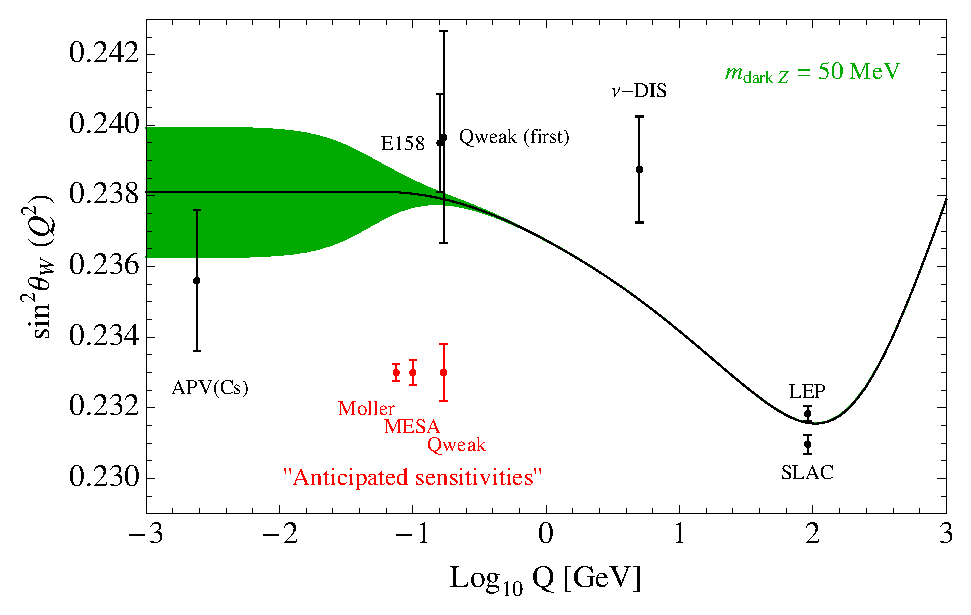
\includegraphics[width=\columnwidth]{fig_running_weinberg_50.eps}
    \caption{Running of the Weinberg angle $\sin^2 \theta_W$ as a function of momentum scale $Q^2$, along with measured values. A deviation from Standard Model predictions (black line) could indicate the presence of new physics effects. The green band indicates the effect of a new $Z'$ with $m_{Z'} = 50 \,\textrm{MeV}$, where the width of the band is determined by the strength of the kinetic mixing parameter with $U(1)_Y$. An $\mathcal{O}$(tonne-year) xenon dark matter observatory can extend the reach of these measurements down to the keV~scale, significantly to the left of this plot, via the measurement of the pp solar neutrino flux. Figure from~\cite{Davoudiasl:2014kua}.}
    \label{fig:weinberg}
\end{figure}

\subsubsection{Electron-Type Neutrino Survival Probability}

The total electron-neutrino scattering rate receives neutral-current contributions from all three flavors, but charge-current contributions only from the electron-type neutrino. Consequently, a high-statistics observation of solar pp neutrinos enables a liquid xenon experiment to directly measure the oscillation probability of the electron-type neutrinos emitted from the Sun in an energy range that is not accessible to any other experiment. \autoref{fig:nusurvival} shows that with an exposure of 300\,tonnes-years, a liquid xenon detector would measure the low-energy survival probability to 3--4\%~\cite{Aalbers:2020gsn}. Such a measurement would serve as a test of the MSW-LMA solution of neutrino oscillation and a probe of exotic neutrino properties and non-standard interactions.

\begin{figure}[!htbp]
    \centering
    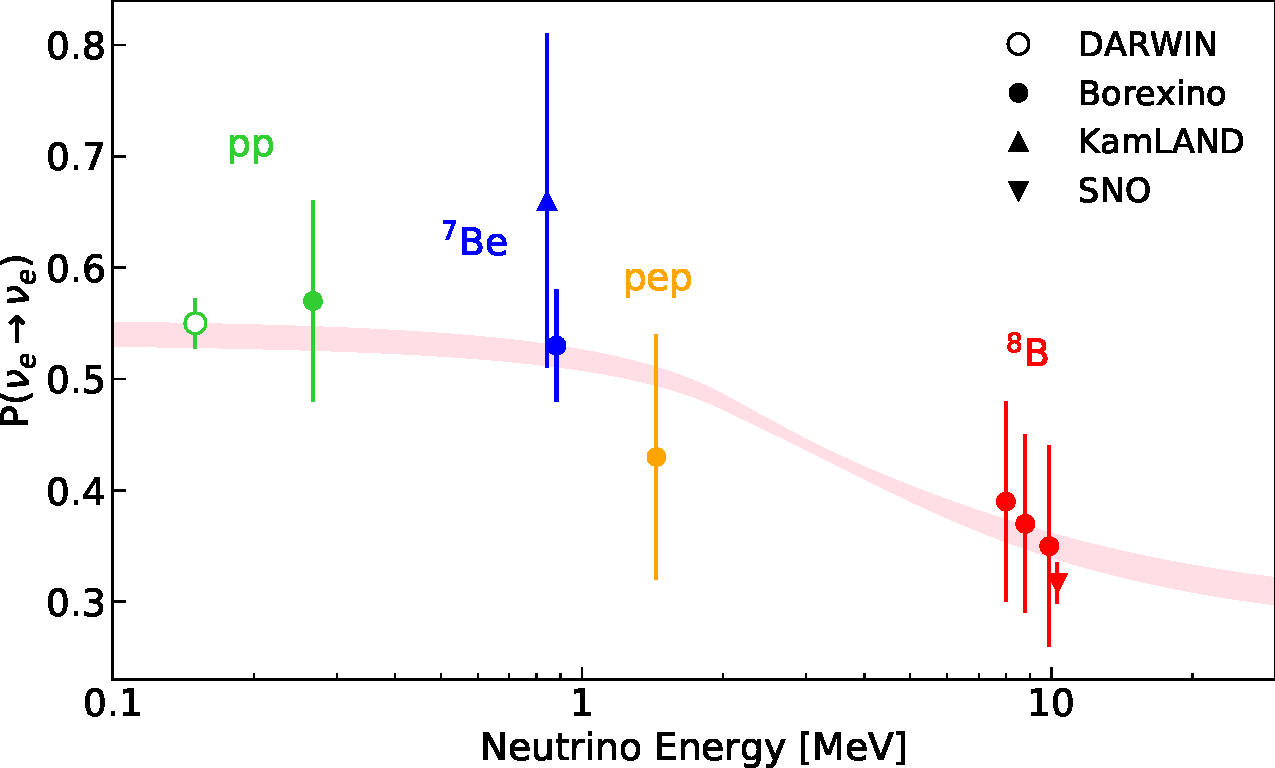
\includegraphics[width=\columnwidth]{fig_nu_surv_vs_energy.pdf}
    \caption{The $\nu_e$ survival probability versus neutrino energy, assuming the high-Z SSM. Dots represent the solar measurements of pp (green), $^7$Be (blue), $pep$ (orange), and $^8$B (red) from Borexino. The upward (downward) triangle shows a measurement of $^7$Be ($^8$B) from KamLAND (SNO). The open point indicates that a next-generation liquid xenon experiment could enhance the precision of the $\nu_e$ survival probability to 0.02 below 200\,keV, using solar pp neutrino events. The pink band represents the 1$\sigma$ prediction of the MSW-LMA solution. Figure from~\cite{Aalbers:2020gsn}.}
    \label{fig:nusurvival}
\end{figure}

\subsubsection{Searching for New Physics of Neutrinos}

A next-generation liquid xenon detector will also be a powerful tool to search for new physics of neutrinos via elastic neutrino-electron scattering. An extensively-studied scenario of new physics of neutrinos is the so-called non-standard interaction (NSI)~\cite{Dev:2019anc}, which might play a potentially important role in future long-baseline experiments such as DUNE~\cite{deGouvea:2015ndi}. In addition, there has also been rising interest in new interactions mediated by light mediators~\cite{Datta:2017ezo,AristizabalSierra:2020edu,Khan:2020vaf}. It has been shown that when combined with a radioactive source, a multi-tonne-scale liquid xenon detector can significantly improve current bounds on leptonic NSIs~\cite{Link:2019pbm} and light mediators, thanks to the high electron density in liquid xenon. In addition, xenon nuclei lie in a range where radiative corrections are particularly sensitive to new weak isospin conserving processes from new physics and are insensitive to isospin violating processes~\cite{Krauss:1991ba}.  Considering solar neutrinos as the source, since the Borexino experiment has demonstrated excellent sensitivities to such new interactions~\cite{Khan:2019jvr, Kamada:2015era}, especially to $\nu_{\tau}$ interactions, it is expected that a next-generation liquid xenon detector will be superior in searching for new physics of neutrinos~\cite{Dutta:2020che}.

